\documentclass[fleqn]{article}
\oddsidemargin 0.0in
\textwidth 6.0in
\thispagestyle{empty}
\usepackage{import}
\usepackage{amsmath}
\usepackage{graphicx}
\usepackage{flexisym}
\usepackage{amssymb}
\usepackage{bigints} 
\usepackage[english]{babel}
\usepackage[utf8x]{inputenc}
\usepackage{float}
\usepackage[colorinlistoftodos]{todonotes}

\definecolor{hwColor}{HTML}{AD53BA}

\begin{document}

  \begin{titlepage}

    \newcommand{\HRule}{\rule{\linewidth}{0.5mm}}

    \center


    \textsc{\LARGE Arizona State University}\\[1.5cm]

    \textsc{\LARGE Classical Parts/Field/Matter I}\\[1.5cm]


    \begin{figure}
      
\includegraphics[width=\linewidth]{asu.png}
    \end{figure}


    \HRule \\[0.4cm]
    { \huge \bfseries Homework Three}\\[0.4cm] 
    \HRule \\[1.5cm]

    \textbf{Behnam Amiri}

    \bigbreak

    \textbf{Prof: Maulik Parikh}

    \bigbreak


    \textbf{{\large \today}\\[2cm]}

    \vfill

  \end{titlepage}

  \begin{enumerate}
    \item Fermat’s principle says that, in traveling between two points, light takes
    the path that minimizes the total travel time. The speed of light in a
    medium with refractive index n is c/n, where c is the speed of light in
    vacuum. Show that, in passing from one medium to another, Fermat’s
    principle implies Snell’s law:
    $$n_1 sin(\theta_1)=n_2 sin(\theta_2)$$ \\
    Where $\theta_i$ are the angles with respect to the normal of the plane of
    interface in the two media. You may assume for simplicity (though it
    is not necessary) that light travels in straight lines within each medium.

      \textcolor{hwColor}{
        Let's start off with finding the times that takes to travel in both
        mediums. \\
        \\
        $
          r=vt \Rightarrow t=\dfrac{r}{v}
        $ 
        \\
        \\
        The total $t$ for the two mediums: \\
        \\
        $
          t=\dfrac{n_1}{c}\sqrt{x^2_1+y^2_1}+\dfrac{n_2}{c} \sqrt{x^2_2+(h-y_1)^2} \\
          \\
          \\
          \dfrac{dt}{dy_1}=\dfrac{d}{dy_1}\left[\dfrac{n_1}{c}\sqrt{x^2_1+y^2_1}+\dfrac{n_2}{c} \sqrt{x^2_2+(h-y_1)^2}\right] \\
          \\
          \\
          =\dfrac{n_1}{c} \dfrac{d}{dy_1} \left[\sqrt{x^2_1+y^2_1}\right]+\dfrac{n_2}{c} \dfrac{d}{dy_1} \left[\sqrt{x^2_2+(h-y_1)^2}\right] \\
          \\
          \\
          =\dfrac{n_1}{c}\left[\dfrac{y_1}{\sqrt{x^2_1+y_1^2}}\right]    +\dfrac{n_2}{c} \left[\dfrac{-(h-y_1)}{\sqrt{x^2_2+(h-y_1)^2}}\right] \\
          \\
          \\
          \\
          \therefore ~~~ n_1 sin(\theta_1)=n_2 sin(\theta_2) \\ \\
        $
        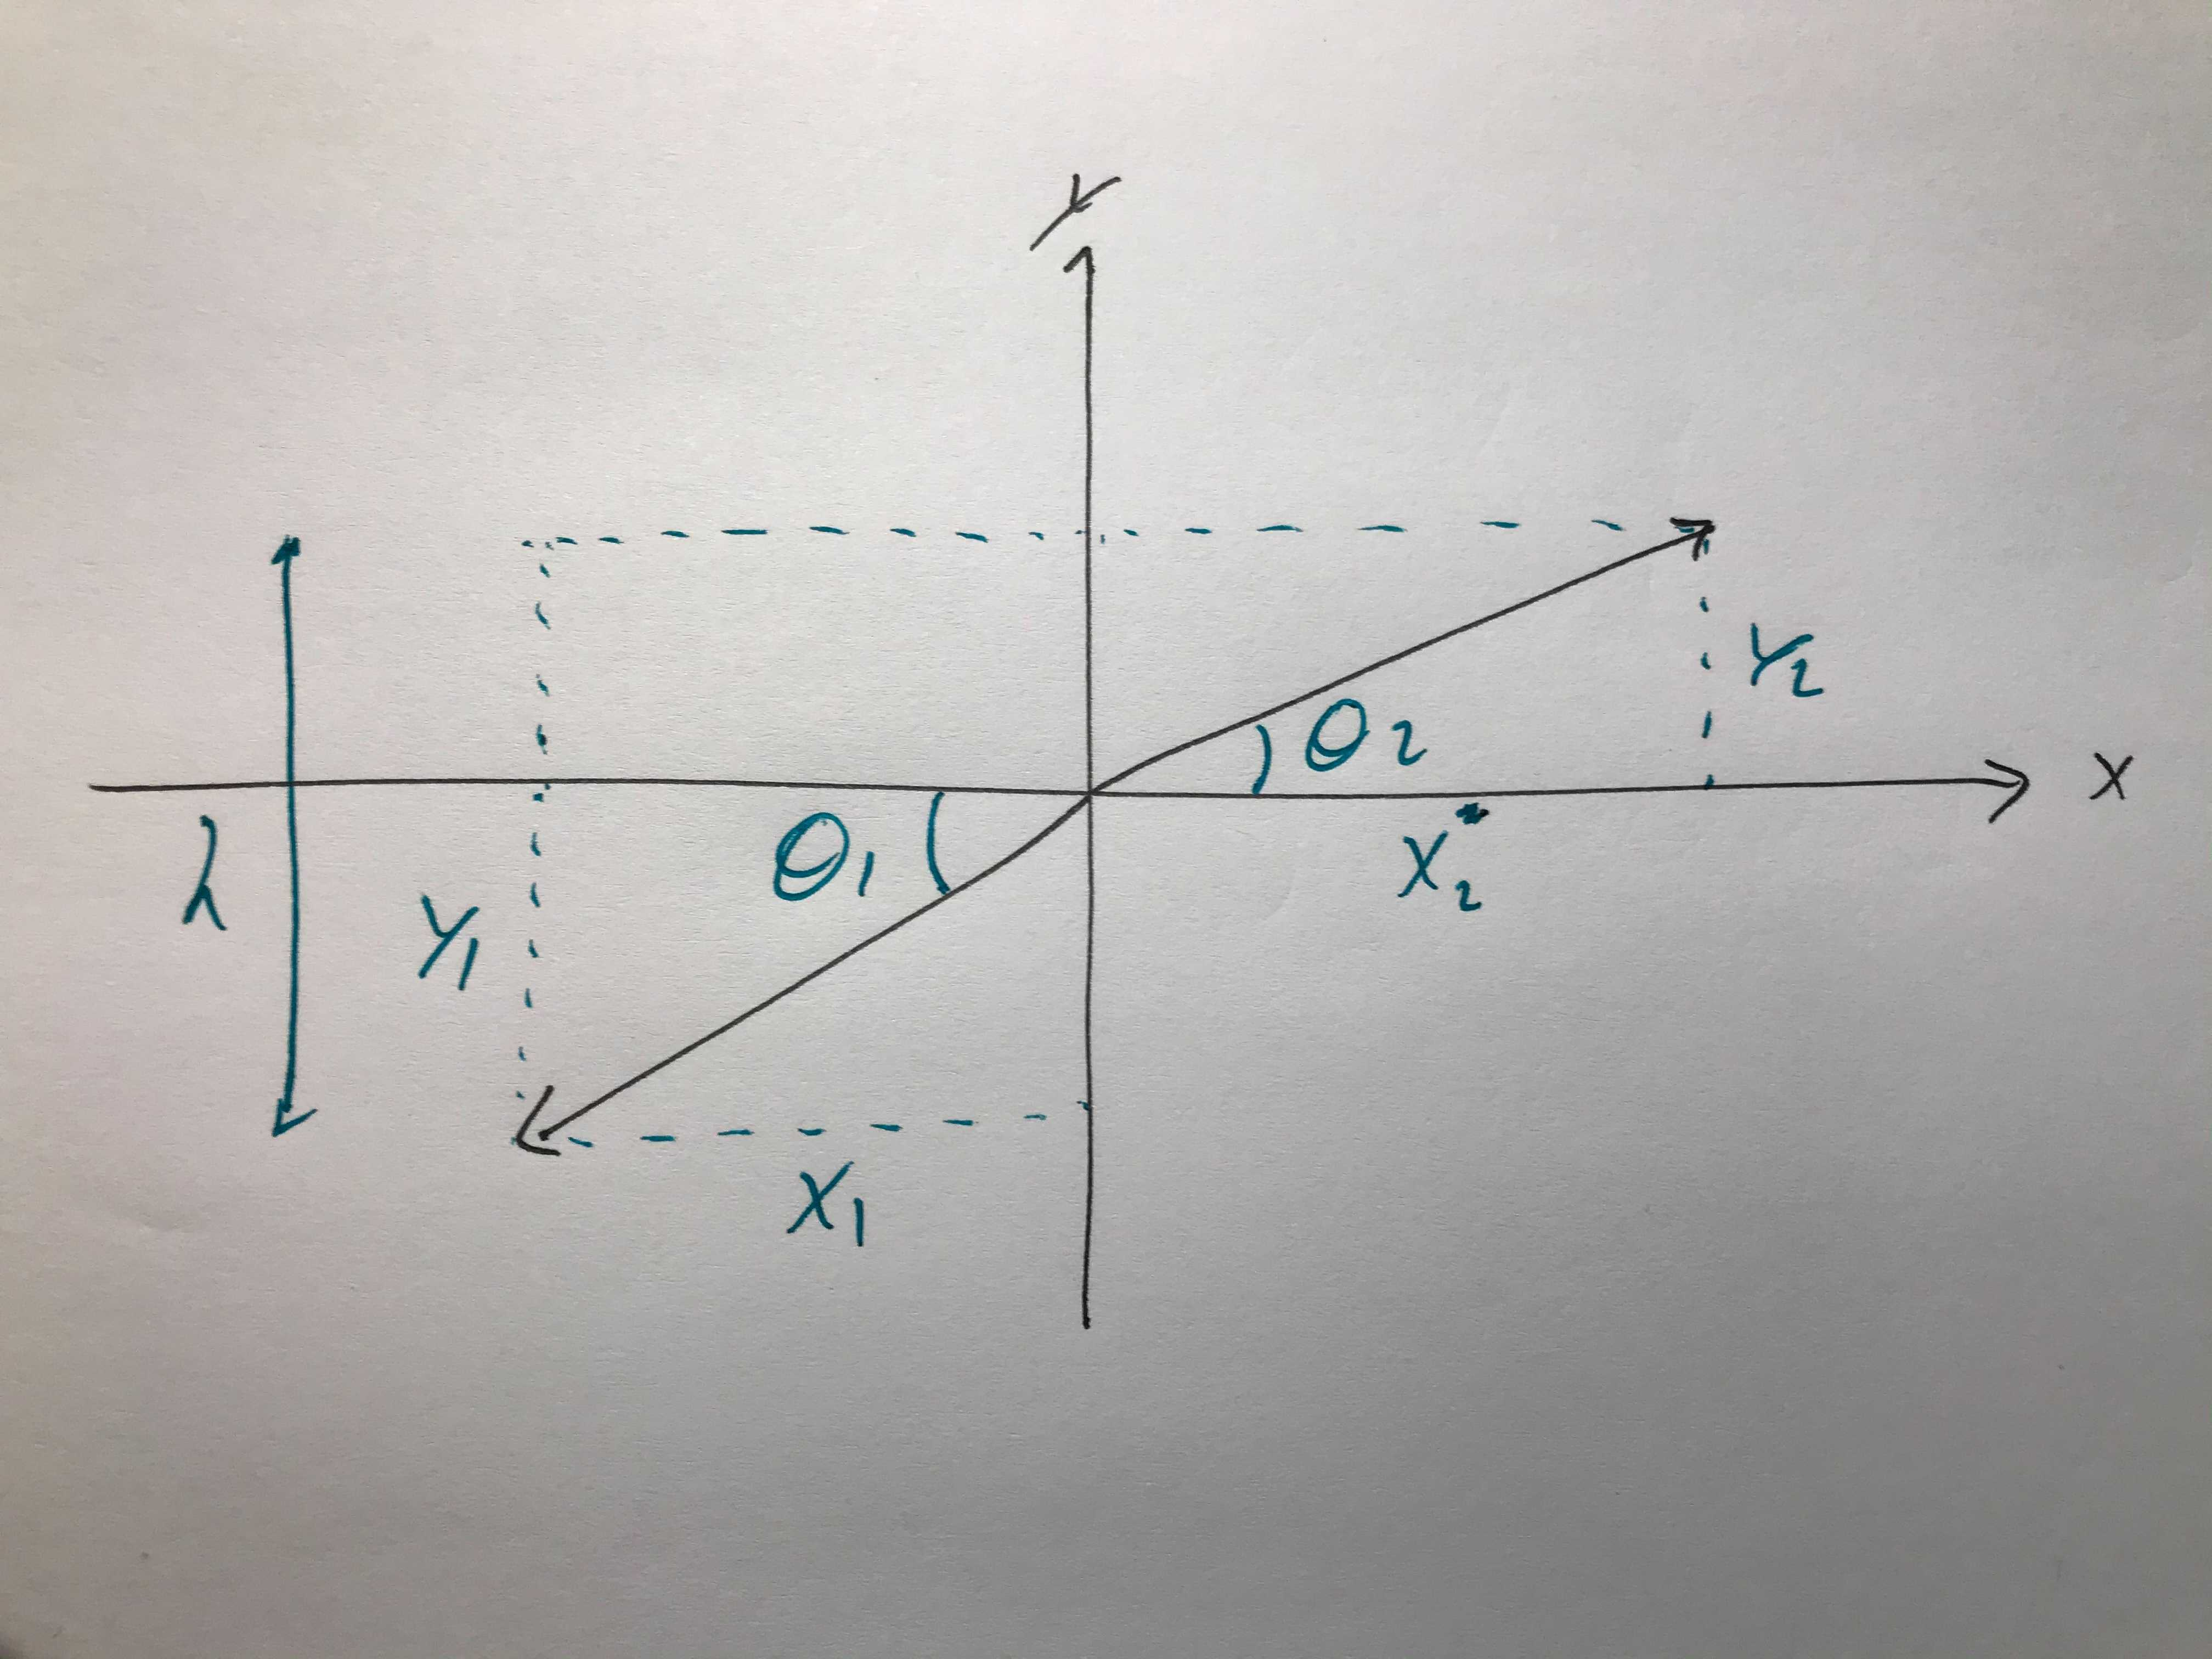
\includegraphics[height=5cm, width=9cm]{n.jpg} 
        \\
      }

    \item Consider a cylinder of radius $R$, parameterized by $0\preceq \theta \preceq 2\pi$ and $z$.
    Find a functional, $L\left[\theta(z)\right]$  for the arc-length of a path $\theta(z)$
    drawn on the cylinder connecting the points $(0,0)$ with $(\theta_0, z_0)$ (where you can
    assume $\theta_0 < \pi$ and $z_0 >0$). Use the Euler-Lagrange equations to find
    the shortest path between those two points on the cylinder.

    \item We’ve seen that harmonic oscillator solutions can be expressed as: 
    $$
    x(t)=C_1 e^{i\omega t}+C_2 e^{-i \omega t} \\
    =A cos(\omega t-\delta) \\
    =B_1 cos(\omega t)+B_2 sin(\omega t) \\
    =Re\{\tilde{A} \}
    $$

    Determine how the coefficients in every line can be expressed in terms
    of those of the following line (expressing the last line in terms of the
    coefficients in the first line).

    \item You are driving a car on a road with bumps every $30 ~ m$. If the car’s
    suspension has a resonant frequency of $0.5 ~ Hz$, at what speed would
    you have to drive in order to experience violent shaking of the car?


    \item A block of mass $m$ sliding horizontally on a frictionless table at velocity
    v strikes a spring of spring constant $k$. The block compresses the spring
    and then bounces back with opposite velocity. How long is the mass in
    contact with the spring? Find the maximum compression of the spring.


    \item A pair of masses, $m$, with positions $x_1$ and $x_2$ are connected by a spring
    of spring constant k and resting length l0 (at which the spring exerts no
    force). Write down the Lagrangian. You can assume $x_2 ≥ x_1$. Find the
    equations of motion. Re-write the Lagrangian in terms of another set
    of generalized coordinates in which the equations are easier to solve.

    \item The curve of a playground slide is defined by the function $z = f(x)$.
    Write down the Lagrangian for a child of mass m going down the slide
    in terms of the variable $x(t)$.

    
    \item  A particle of mass $m$ moving in three dimensions is subject to a potential energy function U(x, y). What is the Lagrangian? Which coordinate is cyclic? What momentum is conserved? If U(x, y) is a function
    only of the combination $x^2 + y^2$ , what other quantity is conserved?

    \item The Lagrangian for a relativistic free particle of rest mass m moving in
    one dimension is
    $$L=-mc\sqrt{c^2-\dot{x}^2}$$
    where c is the speed of light. What is the relativistic equation of motion? Show that, in the non-relativistic limit
    $\dot{x}^2 <<c^2$, this Lagrangian is equivalent to the familiar non-relativistic kinetic energy.   

    \item A bead of mass $m$ slides frictionlessly on a circle of wire with radius R.
    The circle stands up in a vertical plane and rotates about the z-axis
    with constant angular velocity $\omega$. Write down the Lagrangian. Find
    the equations of motion. For an angular velocity greater than some
    critical angular velocity $\omega_c$, the bead will experience small oscillations
    about some stable equilibrium point $\theta_0$. Find $\omega_c$ and $\theta_0(\omega)$.
  \end{enumerate}

\end{document}
